\section*{Learning Objectives}

\begin{itemize}
\item  What is an \texttt{if\,statement} and how to use it
\item A better way to build your own functions
\item A key step in Lower-Upper (LU) Matrix Factorization
\item Debugging, or finding and fixing errors in your code
\end{itemize}

\section*{Outcomes} 
\begin{itemize}
\item Understand how to use Booleans
\item Ability to control program flow via conditional statements
\item Keywords \texttt{if}, \texttt{else}, \texttt{elseif}, and \texttt{end} 
\item Keywords \texttt{function}, \texttt{return}, and \texttt{end} 
\item How to peel off the top row and left-most column of a matrix.
\item (Optional Read) How to compute more easily the area of a general triangle 

\end{itemize}

\vspace*{1cm}

\textbf{Either download Lab4 from our Canvas site or open up a Jupyter notebook so that you can enter code as we go. It is suggested that you have line numbering toggled on.}  

\newpage

\section{If Statements aka Conditional Statements}

\begin{figure}[htb]%
\centering
\subfloat[]{%
    \label{fig:Regression01}%
	\centering
		\setlength{\fboxsep}{0pt}%
\setlength{\fboxrule}{3pt}%
	\fbox{
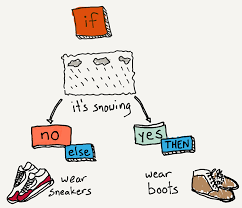
\includegraphics[width=0.3\columnwidth]{Chap04/IfThenElseWearBoots.png}}%
}
\hspace{5pt}%
\subfloat[]{%
    \label{fig:LiDARmap01}%
	\centering
	\setlength{\fboxsep}{0pt}%
\setlength{\fboxrule}{3pt}%
\fbox{
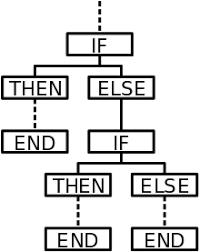
\includegraphics[width=0.3\columnwidth]{Chap04/IfThenEleseWikipedia.png}}%
}
\hspace{5pt}%
\subfloat[]{%
    \label{fig:Regression02}%
	\centering
		\setlength{\fboxsep}{0pt}%
\setlength{\fboxrule}{3pt}%
	\fbox{
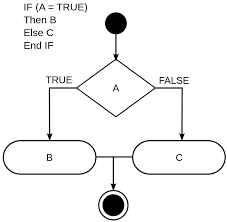
\includegraphics[width=0.32\columnwidth]{Chap04/IfThenEleseWikipedia2.png}}%
}

\caption[]{If statements are also called conditional statements. They allow you to test for a condition before executing a section of code, such as making a recommendation of apparel as a function of the weather. The conditions are always \texttt{\bf T/F} tests. (a) is from \url{https://makecode.microbit.org/courses/csintro/conditionals/overview}, while (b) and (c) are from \url{https://en.wikipedia.org/wiki/Conditional_(computer_programming)}}
    \label{fig:IfThenElse}
\end{figure}


``In computer science, conditionals (that is, conditional statements, conditional expressions and conditional constructs,) are programming language commands for handling decisions;''  see \url{https://en.wikipedia.org/wiki/Conditional_(computer_programming)}. A simple example would be to check for a zero in a denominator before doing a division operation.\\

Julia provides a variety of control flow constructs. Control flow regulates the order of statements to be executed. `if-else` is a common control flow in Julia and other programming languages. The syntax is as follows:
\begin{align*}
if~~ & \textbf{Boolean is \textbf{T}}   \\
& **\texttt{Execute statement block} 1** \\
& **\texttt{Execute statement block} 1** \\
else\\    
& **\texttt{Execute statement block} 2** \\
& **\texttt{Execute statement block} 2** \\
& ** \texttt{Execute statement block} 2** \\
end
\end{align*}

\begin{rem}
Note that in Julia, as in MATLAB, \texttt{\bf then} never appears as a key word! It is implied. 
The first \textbf{true ``if'' or ``elseif''} condition is executed, and then the entire block of \textbf{if statements} is exited. Nothing further is evaluated. If you do not include an \textbf{else} before the end statement, then, if all of the \textbf{if condtions} fail, nothing will be done. This is often very useful, for example, when checking for potential errors in the incoming data to a function. 
\end{rem}

\begin{lstlisting}[language=Julia,style=mystyle]
if (Boolean 1)
    **statement block 1**
elseif (Boolean 2)
    **statement block 2**
elseif (Boolean 3)
    **statement block 3**
...
elseif (Boolean N-1)
    **statement block N-1**
else # nothing goes here
    **statement block N**
end
\end{lstlisting}
% \textbf{Output} 
% \begin{verbatim}

% \end{verbatim}


\begin{lstlisting}[language=Julia,style=mystyle]
# Our first if then else statement
#
# If the condition is evaluated to be true, execute statement1, 
# otherwise, execute statement2
x = sqrt(2)
y = pi/2
if x < y # testing the Boolean (x < y)
    println("x is less than y")
else
    println("x is not less than y")
end
\end{lstlisting}
\textbf{Output} 
\begin{verbatim}
x is less than y
\end{verbatim}

You can string together multiple Boolean conditions, like so. 

\begin{lstlisting}[language=Julia,style=mystyle]
# More conditions can be evaluated using elseif
x = 1
y = 1
if x < y
    println("x is less than y")
elseif x > y
    println("x is greater than y")
else
    println("x is equal to y")
end
\end{lstlisting}
\textbf{Output} 
\begin{verbatim}
x is equal to y
\end{verbatim}

And it is OK to skip the \texttt{else} statement. 


\begin{lstlisting}[language=Julia,style=mystyle]
# It is optional to include the else 
#
x = 1.4142-sqrt(2)
y = NaN
if x < 0
    y = -x
end
[x y]
\end{lstlisting}
\textbf{Output} 
\begin{verbatim}
1×2 Matrix{Float64}:
 -1.35624e-5  1.35624e-5
\end{verbatim}

\begin{example}
Write an ``if statement'' that tests if a variable \texttt{x} is a 1-element vector or not, and when it is a 1-element vector, redefines it as a scalar.
\end{example}

\textbf{Solution}
We first test the \texttt{length} of \texttt{x}. When the length is greater than one, we do nothing. If the length equals one, we then test if \texttt{x} has \texttt{Type} Vector. If it does, we extract its first element to create a scalar.\\


\begin{lstlisting}[language=Julia,style=mystyle]
x=[pi]
# x = pi # uncomment and run, comparing to x = [pi]
@show string(typeof(x))
@show string(typeof(x))[1:6]
if length(x) == 1
    if string(typeof(x))[1:6] == "Vector" # Double equals means EQUIVALENT TO
        @show x=x[1]
        @show typeof(x)
    else
        @show x
    end
end
x
\end{lstlisting}
\textbf{Output} 
\begin{verbatim}
string(typeof(x)) = "Vector\{Irrational\{:\pi\}\}"
(string(typeof(x)))[1:6] = "Vector"
x = x[1] = \pi
typeof(x) = Irrational\{:\pi\}

\pi = 3.1415926535897...
\end{verbatim}

\section{Writing Better Functions}

``A function is a block of organized code that is used to perform a single task. [Functions] provide better modularity for your application and reuse-ability. Depending on the programming language, a function may be called a subroutine, a procedure, a routine, a method, or a subprogram. The generic term, callable unit, is sometimes used. Using functions can allow you to be able to keep your code clean and organized, making it easy to read, and allows the debugging process to be easier;'' from 
\url{https://en.wikiversity.org/wiki/Programming_Fundamentals/Functions}.\\

In Julia, the keywords are \texttt{function}, \texttt{return}, and \texttt{end}. Here we show a very simple function that takes in a variable $x$ and returns $y= x + \pi x^2$.

\begin{lstlisting}[language=Julia,style=mystyle]
# A simple function using the keywords FUNCTION, END, and RETURN
function f(x)
    y = x+pi*x^2
    return y
end
# Call the function
f(2)
\end{lstlisting}
\textbf{Output} 
\begin{verbatim}
14.566370614359172
\end{verbatim}

You can also return more than one value, as in the following example, which also illustrates that any commands that follow the first \texttt{return} statement are ignored.\\

\begin{lstlisting}[language=Julia,style=mystyle]
#
function f(x)
    y = x+pi*x^2
    z = sin(x) + 27*x^3
    return y,z
    w=x+2 # a superfluous line that will be completely ignored 
end
# All operations after the return keyword will be ignored
#
# Call the function
f(3)
\end{lstlisting}
\textbf{Output} 
\begin{verbatim}
(31.274333882308138, 729.1411200080598)
\end{verbatim}

Here is a function that determines the absolute value of a scalar.  \\

\begin{lstlisting}[language=Julia,style=mystyle]
# Build your own absolute value function
function myAbs(a)
    if a >= 0
        return a
    else
        return -a
    end
end
# Call the function
@show myAbs(-2)
@show myAbs(-2.0)
\end{lstlisting}
\textbf{Output} 
\begin{verbatim}
myAbs(-2) = 2
myAbs(-2.0) = 2.0

2.0
\end{verbatim}
Julia has its own built-in \texttt{maximum} function. We'll build our own function just to show how it can be done.

\begin{lstlisting}[language=Julia,style=mystyle]
# Define a more useful function with multiple returns
function myMax(input_vector)
    # initialize the max to the first element 
    # then update when we find a bigger element
    maximum_value = input_vector[1]
    maximum_index = 1
    for i = 1:length(input_vector)
        if input_vector[i] > maximum_value
            maximum_value = input_vector[i]
            maximum_index = i
        end
    end
    return maximum_value, maximum_index
end
\end{lstlisting}
\textbf{Output} 
\begin{verbatim}
myMax (generic function with 1 method)
\end{verbatim}

When we test it, we obtain the maximum value as well as the index of the vector where the maximum value is stored. 
\begin{lstlisting}[language=Julia,style=mystyle]
# Test the function
a = [0, 1, 5, 3.0]
maximum_value, maximum_index = myMax(a)
\end{lstlisting}
\textbf{Output} 
\begin{verbatim}
(5.0, 3)
\end{verbatim}

What if we use a single variable name for the output of the function? 
\begin{lstlisting}[language=Julia,style=mystyle]
# Test the function
a = [0, 1, 5, 3.0]
Answer = myMax(a)
\end{lstlisting}
\textbf{Output} 
\begin{verbatim}
(5.0, 3)
\end{verbatim}

Then \texttt{Answer} is a \texttt{Tuple}. Note that \texttt{Answer[1]} holds the maximum value and \texttt{Answer[2]} holds the index.\\

\begin{lstlisting}[language=Julia,style=mystyle]
@show Answer[1]
Answer[2]
\end{lstlisting}
\textbf{Output} 
\begin{verbatim}
Answer[1] = 5.0

3
\end{verbatim}

\section{A Function for Multiplying Matrices}

Julia has a built-in matrix multiplication function, $A*B$. Just for practice, we'll build a function that uses the method of Chapter 4 in our textbook, where we sum over the product of the columns of $A$ times the rows of $B$.  We will then verify that our function gives the same answer as the usual method of doing matrix multiplication. 

\begin{lstlisting}[language=Julia,style=mystyle]
function myMatrixMultiply(A,B)
    nRowsA, nColsA = size(A)
    nRowsB, nColsB = size(B)
    if nColsA != nRowsB
        println("Error: Matrix sizes are not compatible for multiplication")
        C=NaN
        return C
    end
    C=zeros(nRowsA,nColsB)
    for i = 1:nColsA
        C = C + A[:,i]*B[i:i,:]
    end
    return C
end
\end{lstlisting}
\textbf{Output} 
\begin{verbatim}
myMatrixMultiply (generic function with 1 method)
\end{verbatim}


\begin{lstlisting}[language=Julia,style=mystyle]
# test of myMatrixMultiply(A,B)
using Random
Random.seed!(4321)
A=randn(3,4)
B=randn(4,5)

C=myMatrixMultiply(A,B)
# Matrix of zeros means we got it right!
C-A*B  
\end{lstlisting}
\textbf{Output} 
\begin{verbatim}
3×5 Matrix{Float64}:
  0.0          2.22045e-16  0.0   0.0           0.0
 -1.11022e-16  0.0          0.0   0.0           1.11022e-16
  0.0          0.0          0.0  -2.22045e-16  -5.55112e-17
\end{verbatim}

The next function implements matrix multiplication the way it is done in Julia.\\


\begin{lstlisting}[language=Julia,style=mystyle]
function myMatrixMultiplyOrdinary(A,B)
    nRowsA, nColsA = size(A)
    nRowsB, nColsB = size(B)
    if nColsA != nRowsB
        println("Error: Matrix sizes are not compatible for multiplication")
        C=NaN
        return C
    end
    C=zeros(nRowsA,nColsB)
    for i = 1:nRowsA
        for j = 1:nColsB
            C[i,j] = (A[i:i,:]*B[:,j])[1]
        end
    end
    return C
end
\end{lstlisting}
\textbf{Output} 
\begin{verbatim}
myMatrixMultiplyOrdinary (generic function with 1 method)
\end{verbatim}


\begin{lstlisting}[language=Julia,style=mystyle]
# test of myMatrixMultiplyOrdinary(A,B)
using Random
Random.seed!(4321)
A=randn(3,4)
B=randn(4,5)

C=myMatrixMultiplyOrdinary(A,B)
# Matrix of zeros means we got it right!
C-A*B
\end{lstlisting}
\textbf{Output} 
\begin{verbatim}
3×5 Matrix{Float64}:
  0.0          0.0  0.0  0.0  0.0
 -1.11022e-16  0.0  0.0  0.0  0.0
  0.0          0.0  0.0  0.0  0.0
\end{verbatim}




\section{Forward Substitution}

This is how to solve $Ax = b$ when $A$ is a square lower triangular matrix, with no zeros on the diagonal. See Chapter 3 of the ROB 101 Textbook.

\begin{lstlisting}[language=Julia,style=mystyle]
using LinearAlgebra
function forwardsub(L, b)
    # Assert no entries on the diagonal of U
    # are 0 (or very close to 0)
    @assert minimum(abs.(diag(L))) > 1e-4
    # START of our computations
    n = length(b)
    x = Vector{Float64}(undef, n); #initialize vector x to the correct size
    x[1] = b[1]/L[1,1] #find the first entry of x
    for i = 2:n #find every entry from the 2nd to the end
        x[i]=( b[i] - (L[i,1:i-1])'*x[1:i-1] )/L[i,i] 
        #notice that we used a transpose operator to get the row of L
    end
    # END of our computations.
    return x
end
\end{lstlisting}
\textbf{Output} 
\begin{verbatim}
forwardsub (generic function with 1 method)
\end{verbatim}

Here we work an example with 300 variables. \\


\begin{lstlisting}[language=Julia,style=mystyle]
using Random
Random.seed!(4321)
N=300
L=rand(N,N)
for i = 1:N
    L[i,(i+1):N] = 0.0 * L[i,(i+1):N]
    L[i,i]=1.0
end
b=randn(N,1)
x=forwardsub(L, b)
#x = inv(L)*b
norm(L*x-b)
\end{lstlisting}
\textbf{Output} 
\begin{verbatim}
1.303218919812078e-9
\end{verbatim}


\begin{figure}[htb!]%
\centering
\subfloat[]{%
    \label{fig:Regression03}%
	\centering
		\setlength{\fboxsep}{0pt}%

\includegraphics[width=0.31\columnwidth]{graphics/Chap04/PeelOnion1.png}}%
\hspace{5pt}%
\subfloat[]{%
    \label{fig:LiDARmap03}%
	\centering

\includegraphics[width=0.30\columnwidth]{Chap04/PeelOnion2.png}}%
\hspace{5pt}%
\subfloat[]{%
    \label{fig:Regression04}%
	\centering
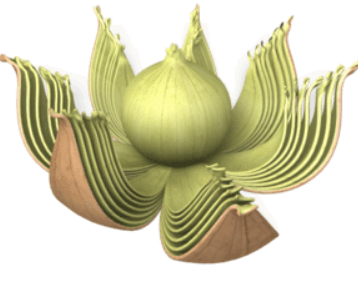
\includegraphics[width=0.31\columnwidth]{Chap04/PeelOnion3.png}}%


\caption[]{We will take a matrix apart, row by row, column by column, until there is nothbing left but zeros. Images are snapshots from \url{https://content.presentermedia.com/content/animsp/00021000/21530/onion_layers_300_wht.gif}.}
    \label{fig:Onion}
\end{figure}

\section{Peeling the Onion: the Base Step for LU Factorization}
\label{sec:PeelingOnions}

This material is tied to Chapter 5 of the ROB 101 Textbook. ``Peeling the Onion'' is an elementary step in factoring a matrix into the product of a lower triangular matrix $L$ and an upper triangular matrix $U$. We will build a function that peels one layer of a matrix at a time. It will work for the special case that the ``pivot'' element is non-zero. Chapter 5 explains how to modify the process when the ``pivot'' is zero, in case you are curious!\\

Consider the square matrix 
$$M_0=\left[\begin{array}{rrr} 
    1   &  4   &  5 \\
     2  &   9  &  17 \\
     3  &  18  &  58 \end{array}  \right]. $$
Our goal is to find a column vector $C_1$ and a row vector $R_1$ such that  
$$M-C_1 \cdot R_1 = \left[\begin{array}{rrr} 
    0  &  0   &  0 \\
     0  &   \ast &  \ast \\
    0  &  \ast  &  \ast \end{array}  \right], $$   
where $\ast$ denotes ``don't care'' in the sense that we do not care about their particular values. Another way to say this is, we want to zero out the first column and the first row of $M$. That means, $C_1$ and $R_1$ are chosen so that the first column and first row of their matrix product $C_1 \cdot R_1$ match the first column and first row of $M$.\\

To see that this is possible, observe that
\begin{align*}
M_0  =\left[\begin{array}{rrr} 
\RED     1   & \RED   4   & \RED  5 \\
 \RED     2  &   9  &  17 \\
 \RED     3  &  18  &  58 \end{array}  \right] &= \underbrace{\left[
\begin{array}{ccc}
\RED 0.0 & \RED 0.0 & \RED 0.0 \\
\RED 0.0 & 1.0 & 7.0 \\
\RED 0.0 & 6.0 & 43.0 \\
\end{array}
\right]}_{M_1} + \underbrace{\left[
\begin{array}{c}
1.0 \\
2.0 \\
3.0 \\
\end{array}
\right]}_{C_1} \cdot \underbrace{\left[
\begin{array}{ccc}
1.0 & 4.0 & 5.0 \\
\end{array}
\right]}_{R_1} \\
& = \underbrace{\left[
\begin{array}{ccc}
\RED 0.0 & \RED 0.0 & \RED 0.0 \\
\RED 0.0 & 1.0 & 7.0 \\
\RED 0.0 & 6.0 & 43.0 \\
\end{array}
\right]}_{M_1}  + \underbrace{\left[
\begin{array}{ccc}
\RED  1.0 &\RED  4.0 &\RED  5.0 \\
\RED 2.0 & 8.0 & 10.0 \\
\RED 3.0 & 12.0 & 15.0 \\
\end{array}
\right]}_{C_1 \cdot R_1}
\end{align*} 
where we arrive at $M_1$ after \textcolor{red}{\bf  ``Peeling off the First Row and First Column''} of $M_0$.\\

Furthermore, we can write 
\begin{align*}
M_1=\left[
\begin{array}{ccc}
 0.0 &  0.0 &  0.0 \\
 0.0 & \RED 1.0 & \RED 7.0 \\
 0.0 & \RED 6.0 & 43.0 \\
\end{array}
\right] & = \underbrace{\left[
\begin{array}{ccc}
0.0 & 0.0 & 0.0 \\
0.0 & \RED 0.0 & \RED 0.0 \\
0.0 & \RED 0.0 & 1.0 \\
\end{array}
\right]}_{M_2} + \underbrace{\left[
\begin{array}{c}
0.0 \\
1.0 \\
6.0 \\
\end{array}
\right]}_{C_2} \cdot \underbrace{\left[
\begin{array}{ccc}
0.0 & 1.0 & 7.0 \\
\end{array}
\right]}_{R_2} \\
& = \underbrace{
\left[
\begin{array}{ccc}
0.0 & 0.0 & 0.0 \\
0.0 & \RED 0.0 & \RED 0.0 \\
0.0 & \RED 0.0 & 1.0 \\
\end{array}
\right]
}_{M_2}  + \underbrace{
\left[
\begin{array}{ccc}
0.0 & 0.0 & 0.0 \\
0.0 & \RED 1.0 & \RED 7.0 \\
0.0 & \RED 6.0 & 42.0 \\
\end{array}
\right]
}_{C_2 \cdot R_2}
\end{align*}
where we arrive at $M_2$ after \textcolor{red}{\bf ``Peeling off the Second Row and Second Column''} of $M_1$. \\


Finally, we can write 
\begin{align*}
M_2=\left[
\begin{array}{ccc}
0.0 & 0.0 & 0.0 \\
0.0 &  0.0 &  0.0 \\
0.0 &  0.0 & \RED 1.0 \\
\end{array}
\right] & = \underbrace{
\left[
\begin{array}{ccc}
0.0 & 0.0 & 0.0 \\
0.0 & 0.0 & 0.0 \\
0.0 & 0.0 & \RED 0.0 \\
\end{array}
\right]
}_{M_3} + \underbrace{\left[
\begin{array}{c}
0.0 \\
0.0 \\
1.0 \\
\end{array}
\right]}_{C_3} \cdot \underbrace{\left[
\begin{array}{ccc}
0.0 & 0.0 & 1.0 \\
\end{array}
\right]}_{R_3} \\
& = \underbrace{
\left[
\begin{array}{ccc}
0.0 & 0.0 & 0.0 \\
0.0 &  0.0 &  0.0 \\
0.0 &  0.0 & \RED 0.0 \\
\end{array}
\right]
}_{M_3}  + \underbrace{
\left[
\begin{array}{ccc}
0.0 & 0.0 & 0.0 \\
0.0 & 0.0 & 0.0 \\
0.0 & 0.0 & \RED 1.0 \\
\end{array}
\right]
}_{C_3 \cdot R_3}
\end{align*}
where we arrive at $M_3$ after \textcolor{red}{\bf ``Peeling off the Third Row and Third Column''} of $M_2$. Because $M_3$ is the zero matrix, the process stops.\\

We have arrived at 
\begin{align*}
M_0  =\left[\begin{array}{rrr} 
    1   &  4   &  5 \\
    2  &   9  &  17 \\
    3  &  18  &  58 \end{array}  \right] &=\underbrace{\left[
\begin{array}{c}
1.0 \\
2.0 \\
3.0 \\
\end{array}
\right]}_{C_1} \cdot \underbrace{\left[
\begin{array}{ccc}
1.0 & 4.0 & 5.0 \\
\end{array}
\right]}_{R_1} +  \underbrace{\left[
\begin{array}{c}
0.0 \\
1.0 \\
6.0 \\
\end{array}
\right]}_{C_2} \cdot \underbrace{\left[
\begin{array}{ccc}
0.0 & 1.0 & 7.0 \\
\end{array}
\right]}_{R_2}  + \underbrace{\left[
\begin{array}{c}
0.0 \\
0.0 \\
1.0 \\
\end{array}
\right]}_{C_3} \cdot \underbrace{\left[
\begin{array}{ccc}
0.0 & 0.0 & 1.0 \\
\end{array}
\right]}_{R_3} \\
& = \underbrace{\left[
\begin{array}{ccc}
1.0 & 0.0 & 0.0 \\
2.0 & 1.0 & 0.0 \\
3.0 & 6.0 & 1.0 
\end{array}
\right]}_{\begin{array}{ccc}
C_1 & C_2 & C_3 \\
\end{array}} \cdot \left. \left[
\begin{array}{ccc}
1.0 & 4.0 & 5.0 \\
0.0 & 1.0 & 7.0 \\
0.0 & 0.0 & 1.0 \\
\end{array}
\right]\right\} \begin{array}{c}
R_1 \\
R_2 \\
R_3 \\
\end{array} \\
& = L \cdot U
\end{align*} 

\textbf{How do we find the column vectors $C_i$ and the row vectors $R_i$, for $1 \le i \le 3$? We have an algorithm for that.}\\

\begin{lstlisting}[language=Julia,style=mystyle]
function peel_one_layer(Temp, k)
    # k is the layer we are peeling (row and column)
    # Temp is the matrix from which we are
    # peeling the k-th row and k-th column
    # We assume layers 1:k-1 are already zeroed
    pivot = Temp[k, k] # We assume pivot != 0
    C = Temp[:, k] / pivot  # Normalized k-th column
    R = Temp[k:k, :]        # k-th row, no normalization
    Temp = Temp - C*R
    return C, R, Temp
end
\end{lstlisting}
\textbf{Output} 
\begin{verbatim}
peel_one_layer (generic function with 1 method)
\end{verbatim}

Now, let's apply our function.

\begin{lstlisting}[language=Julia,style=mystyle]
M0=[1.0 4 5; 2 9 17; 3 18 58]
C1,R1,M1=peel_one_layer(M0, 1) # layer 1
@show C1
@show R1
M1
\end{lstlisting}
\textbf{Output} 
\begin{verbatim}
C1 = [1.0, 2.0, 3.0]
R1 = [1.0 4.0 5.0]

3×3 Matrix{Float64}:
 0.0  0.0   0.0
 0.0  1.0   7.0
 0.0  6.0  43.0
\end{verbatim}

Note that we ``peeled off'' the first column and row.

\begin{lstlisting}[language=Julia,style=mystyle]
C2,R2,M2=peel_one_layer(M1, 2) # layer 2
@show C2
@show R2
M2
\end{lstlisting}
\textbf{Output} 
\begin{verbatim}
C2 = [0.0, 1.0, 6.0]
R2 = [0.0 1.0 7.0]

3×3 Matrix{Float64}:
 0.0  0.0  0.0
 0.0  0.0  0.0
 0.0  0.0  1.0
\end{verbatim}

Note that we ``peeled off'' the second column and row.

\begin{lstlisting}[language=Julia,style=mystyle]
C3,R3,M3=peel_one_layer(M2, 3) # layer 3
@show C3
@show R3
M3
\end{lstlisting}
\textbf{Output} 
\begin{verbatim}
C3 = [0.0, 0.0, 1.0]
R3 = [0.0 0.0 1.0]

3×3 Matrix{Float64}:
 0.0  0.0  0.0
 0.0  0.0  0.0
 0.0  0.0  0.0
\end{verbatim}

We arrived at a matrix of zeros. Next, we form a lower triangular matrix, $L$\\

\begin{lstlisting}[language=Julia,style=mystyle]
L=[C1 C2 C3]
\end{lstlisting}
\textbf{Output} 
\begin{verbatim}
3×3 Matrix{Float64}:
 1.0  0.0  0.0
 2.0  1.0  0.0
 3.0  6.0  1.0
\end{verbatim}

and an upper triangular matrix, $U$\\
\begin{lstlisting}[language=Julia,style=mystyle]
U = [R1;R2;R3]
\end{lstlisting}
\textbf{Output} 
\begin{verbatim}
3×3 Matrix{Float64}:
 1.0  4.0  5.0
 0.0  1.0  7.0
 0.0  0.0  1.0
\end{verbatim}

We now show that $M_0 = L \cdot U$,\\

\begin{lstlisting}[language=Julia,style=mystyle]
M0-L*U
\end{lstlisting}
\textbf{Output} 
\begin{verbatim}
3×3 Matrix{Float64}:
 0.0  0.0  0.0
 0.0  0.0  0.0
 0.0  0.0  0.0
\end{verbatim}

We can place our function \texttt{peel\_one\_layer(Temp, k)} in a \texttt{for\,loop} to compute an LU Factorization when row permutation is not required.

\begin{lstlisting}[language=Julia,style=mystyle]
function myLU(A)
    Temp = copy(A) # Initialize Temp matrix by 
                #copying the original matrix A
    nRows, nCols = size(Temp) # Get the size of the input matrix
    K = minimum([nRows, nCols])
    # Initialize the lower and upper triangular matrix
    L = zeros(Float64, (nRows, K)) # Using zeros function by
                                # specifying both type and size
    U = zeros(Float64, (K, nCols)) 
    # Here we do the actual factorization
    for k = 1:K
        C, R, Temp = peel_one_layer(Temp, k)
        L[:, k] = C
        U[k:k, :] = R
    end
    return L, U
end
\end{lstlisting}
\textbf{Output} 
\begin{verbatim}
myLU (generic function with 1 method)
\end{verbatim}


\begin{lstlisting}[language=Julia,style=mystyle]
using Random
using LinearAlgebra
Random.seed!(09182022)
A = randn(5, 7)
#
L, U = myLU(A)
\end{lstlisting}
\textbf{Output} 
\begin{verbatim}
([1.0 -0.0 … 0.0 -0.0; 1.3841751352784288 1.0 … 0.0 -0.0; … ; 
1.8240441684383097 1.7669720431792901 … 1.0 -0.0; 
1.1660675070497575 0.4629237529415664 … -0.8475551711339656 1.0], 
[-0.3236905701556438 0.9372755784538437 … -0.009357226530146447 -0.0076384514441543774;
0.0 -2.1005108102249452 … 1.4460922800584077 0.41893233388727713;
… ; 0.0 0.0 … 0.19792290864355966 -0.6285612979102336;
-5.551115123125783e-17 0.0 … -1.3304631421106152 1.0052145594104471])
\end{verbatim}

The above output is hard to read. It is better if you look at \texttt{L} and \texttt{U} in separate cells.

\begin{lstlisting}[language=Julia,style=mystyle]
L
\end{lstlisting}
\textbf{Output} 
\begin{verbatim}
5×5 Matrix{Float64}:
 1.0      -0.0        0.0        0.0       -0.0
 1.38418   1.0        0.0        0.0       -0.0
 8.38948   4.18061    1.0        0.0       -0.0
 1.82404   1.76697    0.271808   1.0       -0.0
 1.16607   0.462924  -0.135905  -0.847555   1.0
\end{verbatim}


\begin{lstlisting}[language=Julia,style=mystyle]
U
\end{lstlisting}
\textbf{Output} 
\begin{verbatim}
5×7 Matrix{Float64}:
 -0.323691      0.937276   0.578516  … 0.487937  -0.00935723  -0.00763845
  0.0          -2.10051   -1.18148      -0.516585   1.44609      0.418932
  0.0           0.0        2.42504      -1.45327   -6.78688     -1.58847
  0.0           0.0        0.0           0.717684   0.197923    -0.628561
 -5.55112e-17   0.0        0.0          -2.41577   -1.33046      1.00521
\end{verbatim}

\begin{lstlisting}[language=Julia,style=mystyle]
A-L*U
\end{lstlisting}
\textbf{Output} 
\begin{verbatim}
5×7 Matrix{Float64}:
 0.0   0.0           0.0          0.0          … 0.0           0.0
 0.0   0.0           0.0          6.93889e-17      0.0           0.0
 0.0  -4.44089e-16  -4.44089e-16  6.66134e-16     -4.44089e-16  -5.55112e-17
 0.0  -4.44089e-16  -1.11022e-16  5.55112e-17      3.33067e-16   0.0
 0.0   1.38778e-17   8.32667e-17  0.0              1.38778e-16   0.0
\end{verbatim}

\section{Debugging}

We'll introduce errors into a few of the functions and if-then-else statements we have used in the Chapter and see how the ``bugs''  manifest themselves. \\

\subsection{Misusing operations designed for scalar variables}
Here is a function designed for $x$ a real number.

\begin{lstlisting}[language=Julia,style=mystyle]
function f(x)
    y = x+pi*x^2
    return y
end
\end{lstlisting}
\textbf{Output} 
\begin{verbatim}
f (generic function with 1 method)
\end{verbatim}

We forget that we designed it for a real number and try to apply it to a vector.

\begin{lstlisting}[language=Julia,style=mystyle]
f([1;2])
\end{lstlisting}
\textbf{Output} 
\begin{verbatim}
MethodError: no method matching ^(::Vector{Int64}, ::Int64)
Closest candidates are:
  ^(::Union{AbstractChar, AbstractString}, ::Integer) at strings/basic.jl:718
  ^(::Complex{var"#s79"} where var"#s79"<:AbstractFloat, ::Integer) at complex.jl:818
  ^(::Complex{var"#s79"} where var"#s79"<:Integer, ::Integer) at complex.jl:820
  ...

Stacktrace:
 [1] macro expansion
   @ ./none:0 [inlined]
 [2] literal_pow
   @ ./none:0 [inlined]
 [3] f(x::Vector{Int64})
   @ Main ./In[1]:2
 [4] top-level scope
   @ In[2]:1
 [5] eval
   @ ./boot.jl:360 [inlined]
 [6] include_string(mapexpr::typeof(REPL.softscope), mod::Module, 
 code::String, filename::String)
   @ Base ./loading.jl:1094

\end{verbatim}

In the above error message, \texttt{top-level scope, ~@ In[1]:2 } is referring to the Cell where we defined the function. The message ``\textcolor{red}{\bf MethodError: no method matching $ \wedge $(::Vector{Int64}, ::Int64)}'' is telling us that Julia does not know how to compute the square of a vector. There are two solutions to this. 


\begin{lstlisting}[language=Julia,style=mystyle]
f.([1;2]) # Solution 1 is to apply broadcasting
\end{lstlisting}
\textbf{Output} 
\begin{verbatim}
2-element Vector{Float64}:
  4.141592653589793
 14.566370614359172
\end{verbatim}

\begin{lstlisting}[language=Julia,style=mystyle]
function f(x)
    y = x .+ pi * x.^2 # Solution 2 is make the function work for vectors or scalars
    return y
end

f([1;2])
\end{lstlisting}
\textbf{Output} 
\begin{verbatim}
2-element Vector{Float64}:
  4.141592653589793
 14.566370614359172
\end{verbatim}

\subsection{Bounds Error}

We recall our function for multiplying matrices.

\begin{lstlisting}[language=Julia,style=mystyle]
function myMatrixMultiply(A,B)
    nRowsA, nColsA = size(A)
    nRowsB, nColsB = size(B)
    if nColsA != nRowsB
        println("Error: Matrix sizes are not compatible for multiplication")
        C=NaN
        return C
    end
    C=zeros(nRowsA,nColsB)
    for i = 1:nColsA
        C = C + A[:,i]*B[i:i,:]
    end
    return C
end

\end{lstlisting}
\textbf{Output} 
\begin{verbatim}
myMatrixMultiply (generic function with 1 method)
\end{verbatim}

We give the function what looks like perfectly good data.

\begin{lstlisting}[language=Julia,style=mystyle]
A=[1 2 3 4]
B=[2;3;4;5.0]
myMatrixMultiply(A,B)
\end{lstlisting}
\textbf{Output} 
\begin{verbatim}
BoundsError: attempt to access Tuple{Int64} at index [2]

Stacktrace:
 [1] indexed_iterate
   @ ./tuple.jl:86 [inlined]
 [2] myMatrixMultiply(A::Matrix{Int64}, B::Vector{Float64})
   @ Main ./In[6]:3
 [3] top-level scope
   @ In[7]:3
 [4] eval
   @ ./boot.jl:360 [inlined]
 [5] include_string(mapexpr::typeof(REPL.softscope), mod::Module, 
 code::String,  filename::String)
   @ Base ./loading.jl:1094
\end{verbatim}

Cell [6] is where we defined the function \texttt{myMatrixMultiply} and line 3 is the command \texttt{nRowsB, nColsB = size(B)}. The problem is that $B$ is a vector and the \texttt{size} command does not return a value for $\rm nColsB$, even though we ``know'' it should be one. \\

In the following, we show two ways to fix this issue. In the first \texttt{if-then-else} statement, we make use of Types in Julia. In the second \texttt{if-then-else} statement, we exploit the fact that if $B$ is a matrix, then \texttt{size(B)} has two components, and hence its length is two, and when $B$ is a vector or scalar, \texttt{size(B)} will have length one. This is certainly the simpler solution of the two. \textcolor{blue}{\bf An even simpler solution is only to call the function with matrix arguments!}  

\begin{lstlisting}[language=Julia,style=mystyle]
function myMatrixMultiply(A,B)
    if (typeof(A) == Matrix{Int64})||(typeof(A) == Matrix{Float64})
        nRowsA, nColsA = size(A)
    else
        nRowsA = length(A)
        nColsA = 1
    end

    if length(size(B)) == 2
        nRowsB, nColsB = size(B)
    else
        nRowsB = length(B)
        nColsB = 1
    end
    if nColsA != nRowsB
        @show nColsA
        @show nRowsB
        println("Error: Matrix sizes are not compatible for multiplication")
        C=NaN
        return C
    end
    C=zeros(nRowsA,nColsB)
    for i = 1:nColsA
        C = C + A[:,i]*B[i:i,:]
    end
    return C
end
\end{lstlisting}
\textbf{Output} 
\begin{verbatim}
myMatrixMultiply (generic function with 1 method)
\end{verbatim}


\begin{lstlisting}[language=Julia,style=mystyle]
myMatrixMultiply(A,B)
\end{lstlisting}
\textbf{Output} 
\begin{verbatim}
1×1 Matrix{Float64}:
 40.0
\end{verbatim}

\subsection{Using the display( ) command to find an error buried in a function}

We insert an error in a function that worked just fine for us in Chapter~\ref{sec:PeelingOnions}. Can you spot the error before we run the function? 

\begin{lstlisting}[language=Julia,style=mystyle]
function peel_one_layer(Temp, k)
# k is the layer we are peeling (row and column)
# Temp is the matrix from which we are
# peeling the k-th row and k-th column
    pivot = Temp[k, k]
    C = Temp[:, k] # kth column
    # next we normalize
    C = C / pivot # We assume pivot != 0
    R = Temp[k, :]  # kth row
    Temp = Temp - C*R
    return C, R, Temp
end
\end{lstlisting}
\textbf{Output} 
\begin{verbatim}
peel_one_layer (generic function with 1 method)
\end{verbatim}

\begin{lstlisting}[language=Julia,style=mystyle]
Temp=[1.0 2; 3 4]
display(Temp)
C, R, Temp = peel_one_layer(Temp, 1)
\end{lstlisting}
\textbf{Output} 
\begin{verbatim}
2×2 Matrix{Float64}:
 1.0  2.0
 3.0  4.0
 
MethodError: no method matching *(::Vector{Float64}, ::Vector{Float64})
Closest candidates are:
  *(::Any, ::Any, ::Any, ::Any...) at operators.jl:560
  *(::StridedMatrix{T}, ::StridedVector{S}) where 
  {T<:Union{Float32, Float64, ComplexF32, ComplexF64}, S<:Real} at
  /buildworker/worker/package_linux64/build/usr/share/julia/stdlib/v1.6/
LinearAlgebra/src/matmul.jl:44
  *(::StridedVecOrMat{T} where T, ::LinearAlgebra.Adjoint{var"#s832", var"#s831"} 
  where {var"#s832", var"#s831"<:LinearAlgebra.LQPackedQ}) at 
  /buildworker/worker/package_linux64/build/usr/share/julia/stdlib
  /v1.6/LinearAlgebra/src/lq.jl:254
  ...

Stacktrace:
 [1] peel_one_layer(Temp::Matrix{Float64}, k::Int64)
   @ Main ./In[49]:10
 [2] top-level scope
   @ In[52]:3
 [3] eval
   @ ./boot.jl:360 [inlined]
 [4] include_string(mapexpr::typeof(REPL.softscope), mod::Module, code::String, 
 filename::String)
   @ Base ./loading.jl:1094
\end{verbatim}

The message \texttt{no method matching *(::Vector{Float64}, ::Vector{Float64})} is telling us that Julia does not know how to multiply two vectors. We are surprised by this message because we think, in line 10 of our function (from the message \texttt{In[49]:10}) that we are multiplying a column vector $C$ times a row vector $R$, which is a legitimate operation. \textcolor{red}{\bf To find the error, we use the \texttt{display} command} (you could also have used the \texttt{@show} command).


\begin{lstlisting}[language=Julia,style=mystyle]
function peel_one_layer(Temp, k)
# k is the layer we are peeling (row and column)
# Temp is the matrix from which we are
# peeling the k-th row and k-th column
    pivot = Temp[k, k]
    C = Temp[:, k] # kth column
    # next we normalize
    C = C / pivot # We assume pivot != 0
    R = Temp[k, :]  # kth row
    display(C)
    display(R)
    Temp = Temp - C*R
    return C, R, Temp
end

C, R, Temp = peel_one_layer(Temp, 1)
\end{lstlisting}
\textbf{Output} 
\begin{verbatim}
2-element Vector{Float64}:
 1.0
 3.0
2-element Vector{Float64}:
 1.0
 2.0
MethodError: no method matching *(::Vector{Float64}, ::Vector{Float64})
\end{verbatim}

Sure enough, $R$ is a column vector. And we note that we should have used \texttt{    R = Temp[k:k, :]} to extract a row and keep it a row.\\

If we use the \texttt{@show} command, we get the same information but it's less direct in that we have to recognize that \texttt{R = [1.0, 2.0]} is a column vector due to the comma separating the two entries.

\begin{lstlisting}[language=Julia,style=mystyle]
function peel_one_layer(Temp, k)
# k is the layer we are peeling (row and column)
# Temp is the matrix from which we are
# peeling the k-th row and k-th column
    pivot = Temp[k, k]
    C = Temp[:, k] # kth column
    # next we normalize
    C = C / pivot # We assume pivot != 0
    R = Temp[k, :]  # kth row
    @show C
    @show R
    Temp = Temp - C*R
    return C, R, Temp
end

C, R, Temp = peel_one_layer(Temp, 1)
\end{lstlisting}
\textbf{Output} 
\begin{verbatim}
C = [1.0, 3.0]
R = [1.0, 2.0]

MethodError: no method matching *(::Vector{Float64}, ::Vector{Float64})
\end{verbatim}


% \begin{lstlisting}[language=Julia,style=mystyle]

% \end{lstlisting}
% \textbf{Output} 
% \begin{verbatim}

% \end{verbatim}

% \begin{lstlisting}[language=Julia,style=mystyle]

% \end{lstlisting}
% \textbf{Output} 
% \begin{verbatim}

% \end{verbatim}

\section{(Optional Read) ``Hero 60 AD'' or Heron's Formula for the Area of a Triangle}


While everyone knows the formula ${\rm Area} = \frac{1}{2} {\rm base} \times {\rm height}$ for the area of a triangle, very few of us were taught Heron's formula, which avoids the use of trigonometry or geometry to compute the height of the triangle (of course, when it is not a right triangle). We create a function using this formula and then illustrate the programming adage, \textbf{``garbage in, garbage out''}. \\

A derivation of Heron's formula can be found here on YouTube \url{https://www.youtube.com/watch?v=9qbpmYqr4so} or in Wikipedia \url{https://en.wikipedia.org/wiki/Heron\%27s_formula}, where it is pointed out that ``The formula is credited to Heron (or Hero) of Alexandria, and a proof can be found in his book Metrica, written around AD 60. It has been suggested that Archimedes knew the formula over two centuries earlier, and since Metrica is a collection of the mathematical knowledge available in the ancient world, it is possible that the formula predates the reference given in that work.'' Moreover, the Chinese had discovered a similar formula, documented in 1247 \url{https://en.wikipedia.org/wiki/Mathematical_Treatise_in_Nine_Sections}, though it may have been known much earlier.


\begin{figure}[htb!]%
\centering
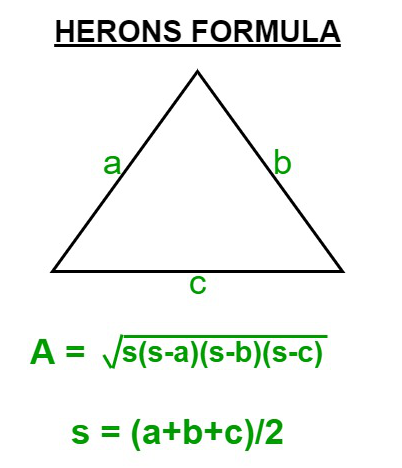
\includegraphics[width=0.31\columnwidth]{graphics/Chap04/heron.jpg}%
\caption[]{Heron's formula for the area of a triangle. Source  \url{https://www.geeksforgeeks.org/herons-formula/}.}
    \label{columneron}
\end{figure}

\begin{lstlisting}[language=Julia,style=mystyle]
function heron(a, b, c)
    s = (a + b + c)/2
    Area = sqrt( s*(s-a)*(s-b)*(s-c) )
    return Area
end
\end{lstlisting}
\textbf{Output} 
\begin{verbatim}
heron (generic function with 1 method)
\end{verbatim}

We now insert the canonical right triangle, (3, 4, 5), where we can take the base as 3 and the height as 2 or the base as 4 and the height as 1.5. In either case, the area is 6.0, and voil\`a, Heron agrees with us! 
\begin{lstlisting}[language=Julia,style=mystyle]
area = heron(3,4,5)
\end{lstlisting}
\textbf{Output} 
\begin{verbatim}
6.0
\end{verbatim}

What about a triangle with side lengths (3, 4, 4.5)? \\

\begin{lstlisting}[language=Julia,style=mystyle]
area = heron(3,4,4.5)
\end{lstlisting}
\textbf{Output} 
\begin{verbatim}
5.881313097429858
\end{verbatim}

Can you correctly compute the area using trigonometry? Go for it! \\

\textcolor{red}{\bf \large Garbage in, garbage out}. What if we insert data into our function where the lengths of the sides are not compatible with forming a triangle, such as (3, 4, 8)?\\

\begin{lstlisting}[language=Julia,style=mystyle]
area = heron(3,4,8)
\end{lstlisting}
\textbf{Output} 
\begin{verbatim}
DomainError with -59.0625:
sqrt will only return a complex result if called with a complex argument. 
Try sqrt(Complex(x)).

Stacktrace:
 [1] throw_complex_domainerror(f::Symbol, x::Float64)
   @ Base.Math ./math.jl:33
 [2] sqrt
   @ ./math.jl:582 [inlined]
 [3] heron(a::Int64, b::Int64, c::Int64)
   @ Main ./In[50]:3
 [4] top-level scope
   @ In[51]:1
 [5] eval
   @ ./boot.jl:360 [inlined]
 [6] include_string(mapexpr::typeof(REPL.softscope), mod::Module, code::String, 
 filename::String)
   @ Base ./loading.jl:1094
\end{verbatim}

The error is on line 3; we tried to take the square root of a negative number. We know if the sum of the two shortest sides exceeds the largest side, then we cannot form a triangle. Let's add this as a check on our function, and while we are at it, also check for negative lengths!\\ 

\begin{lstlisting}[language=Julia,style=mystyle]
function heron(a, b, c)
    # Let's include tests on the inputs to make
    # sure they correspond to a feasible triangle
    #
    data=sort([a; b; c])
    a=data[1]; b=data[2]; c=data[3]
    if a <= 0
        println("Cannot have sides with non-positive length")
        return im # return an imaginary number, just for fun
    elseif c > a + b
        println("Provided data does not form a triangle")
        return im # return an imaginary number, just for fun
    end
    s = (a + b + c)/2 # semi-perimeter
    Area = sqrt( s*(s-a)*(s-b)*(s-c) )
    return Area
end
\end{lstlisting}
\textbf{Output} 
\begin{verbatim}
heron (generic function with 1 method)
\end{verbatim}

The above is a more professional version of our function. \\

\begin{lstlisting}[language=Julia,style=mystyle]
area = heron(3,4,8)
\end{lstlisting}
\textbf{Output} 
\begin{verbatim}
Provided data does not form a triangle

im
\end{verbatim}

The sky is the limit! Here is a version of the function where we can specify the input data in two forms:
\begin{itemize}
    \item as three points in $\real^n$ and then compute the area of the triangle formed by the points, or
    \item as the lengths of the sides, as we did before.
\end{itemize}


\begin{lstlisting}[language=Julia,style=mystyle]
using LinearAlgebra
function heron(A, B, C)
    dim = maximum([length(A), length(B), length(C)])
    if dim > 1
        # Input consists of points in Rn for n >= 2
        if ( length(A) == length(B) )&( length(B) == length(C))
            a=norm(A-B); b = norm(B-C); c = norm(C-A)
            # Lengths will automatically form a triangle
            s = (a + b + c)/2 # semi-perimeter
            Area = sqrt( s*(s-a)*(s-b)*(s-c) )
            return Area
        else
            println("Data is not consistent as points in Rn")
            return im # return an imaginary number, just for fun
        end
    else
        # Input consists of lengths of the sides
        # Check the lengths to make sure
        # they correspond to a feasible triangle
        #
        data=sort([A; B; C])
        a=data[1]; b=data[2]; c=data[3]
        if a <= 0
            println("Cannot have sides with non-positive length")
            return im # return an imaginary number, just for fun
        elseif c > a + b
            println("Provided data does not form a triangle")
            return im # return an imaginary number, just for fun
        end
        s = (a + b + c)/2 # semi-perimeter
        Area = sqrt( s*(s-a)*(s-b)*(s-c) )
        return Area
    end    
end
\end{lstlisting}
\textbf{Output} 
\begin{verbatim}
heron (generic function with 1 method)
\end{verbatim}


\begin{lstlisting}[language=Julia,style=mystyle]
heron([1 2 0], [2 3 5], [4 0 6])
\end{lstlisting}
\textbf{Output} 
\begin{verbatim}
9.513148795220223
\end{verbatim}


% \begin{lstlisting}[language=Julia,style=mystyle]

% \end{lstlisting}
% \textbf{Output} 
% \begin{verbatim}

% \end{verbatim}


% \begin{lstlisting}[language=Julia,style=mystyle]

% \end{lstlisting}
% \textbf{Output} 
% \begin{verbatim}

% \end{verbatim}



\section{(Optional Read) More Examples Combining Functions and Flow Control}



\begin{lstlisting}[language=Julia,style=mystyle]
# Here is a function that takes in a square matrix
# and returns an upper triangular matrix, meaning one that 
# has all zeros BELOW the diagonal
function makeTriangularMat(A)
    B=copy(A)
    nRows, nCols = size(B)
    for k = 2: nRows
        B[k,1:k-1] = 0.0 * B[k,1:k-1]
    end
    return B
end
\end{lstlisting}
\textbf{Output} 
\begin{verbatim}
makeTriangularMat (generic function with 1 method)
\end{verbatim}


\begin{lstlisting}[language=Julia,style=mystyle]
using Random
Random.seed!(4321)
A=randn(5,5)
Atri=makeTriangularMat(A)
\end{lstlisting}

\textbf{Output} 
\begin{verbatim}
5 x 5 Matrix{Float64}:
 -0.229071  -1.95979   -1.00753   -0.0688075   0.673963
  0.0       -0.991273   0.825056   1.51188     0.317936
  0.0       -0.0       -0.850184  -0.718068   -1.13022
  0.0        0.0        0.0       -1.06297    -0.0391889
 -0.0       -0.0       -0.0       -0.0         0.609128
\end{verbatim}


\begin{lstlisting}[language=Julia,style=mystyle]
# Here is a function that takes in a rectangular matrix
# and returns an upper triangular matrix, meaning one that 
# has all zeros BELOW the diagonal
function makeTriangularMat(A)
    B=copy(A)
    nRows, nCols = size(B)
    for k = 2: nRows
        K=minimum([k-1,nCols]) # min of the two numbers
        B[k,1:K] = 0.0 * B[k,1:K]
    end
    return B
end
\end{lstlisting}
\textbf{Output} 
\begin{verbatim}
makeTrinagularMat (generic function with 1 method)
\end{verbatim}


Because of the additional line of code \texttt{K=minimum([k-1, nCols])}, our function \texttt{makeTriangularMat(A)} will now do the correct thing for rectangular matrices. The additional line of code prevents us from indexing into non-existent columns of the matrix because \texttt{K} can never be greater than \texttt{nCols}, the number of columns of our matrix.\\

\begin{lstlisting}[language=Julia,style=mystyle]
# Our code works on non-square matrices
using Random
A=randn(5,4)
Atri=makeTrinangularMat(A)
\end{lstlisting}
\textbf{Output} 
\begin{verbatim}
5×4 Matrix{Float64}:
 -0.535644  -0.11       0.258952  -1.30922
  0.0        0.423592  -1.48126   -1.52763
  0.0       -0.0        1.25757   -0.215213
  0.0        0.0       -0.0        1.99146
 -0.0        0.0       -0.0        0.0
\end{verbatim}


\begin{lstlisting}[language=Julia,style=mystyle]
# Our code works on non-square matrices
using Random
Random.seed!(4321)
A=randn(4,5)
Atri=makeTriangularMat(A)
\end{lstlisting}
\textbf{Output} 
\begin{verbatim}
4 x 5 Matrix{Float64}:
 -0.229071  -0.540755   1.02869  -0.850184    1.51188
  0.0       -1.95979   -1.94117   0.592798   -0.718068
  0.0       -0.0       -1.00753  -0.358643   -1.06297
  0.0       -0.0        0.0      -0.0688075  -0.509626
\end{verbatim}


\begin{lstlisting}[language=Julia,style=mystyle]
# Our code now works on non-square matrices
using Random
Random.seed!(4321)
A=randn(5,4)
Atri=makeTriangularMat(A)
\end{lstlisting}
\textbf{Output} 
\begin{verbatim}
5×4 Matrix{Float64}:
 -0.229071  -1.95979   -1.00753   -0.0688075
  0.0       -0.991273   0.825056   1.51188
  0.0       -0.0       -0.850184  -0.718068
  0.0        0.0        0.0       -1.06297
 -0.0       -0.0       -0.0       -0.0
\end{verbatim}



Our function \texttt{myAbs} only works for scalars. When we try it on a vector, we upset Julia.\\

\begin{lstlisting}[language=Julia,style=mystyle]
myAbs([-pi 2])
\end{lstlisting}
\textbf{Output} 
\begin{verbatim}
MethodError: no method matching isless(::Int64, ::Matrix{Float64})
Closest candidates are:
  isless(::Any, ::Missing) at missing.jl:88
  isless(::Missing, ::Any) at missing.jl:87
  isless(::Real, ::AbstractFloat) at operators.jl:168
  ...

Stacktrace:
 [1] <(x::Int64, y::Matrix{Float64})
   @ Base ./operators.jl:279
 [2] <=(x::Int64, y::Matrix{Float64})
   @ Base ./operators.jl:328
 [3] >=(x::Matrix{Float64}, y::Int64)
   @ Base ./operators.jl:352
 [4] myAbs(a::Matrix{Float64})
   @ Main ./In[3]:3
 [5] top-level scope
   @ In[4]:1
 [6] eval
   @ ./boot.jl:360 [inlined]
 [7] include_string(mapexpr::typeof(REPL.softscope), mod::Module, code::String,
 filename::String)
   @ Base ./loading.jl:1094
\end{verbatim}

\textbf{We will now add in conditional checks to make it work for row vectors and column vectors.} The first thing to ask ourselves, is how to check for a scalar? In the code below, we are checking that our input has length one and is not a \texttt{Vector} or a \texttt{Matrix}! \\



\begin{lstlisting}[language=Julia,style=mystyle]
# Extend the your absolute value function to work on vectors
function myAbs(a)
    B = (string(typeof(a))[1] !== 'V' ) & (string(typeof(a))[1] !== 'M' )
    if (length(a) == 1) & B
        if a >= 0 
            return a
        else
            return -a
        end
    else
        y = copy(a) # Preserves TYPE meaning Vector or row Matrix
        for i=1:length(a)
            if a[i] < 0
                y[i] = -a[i]
            end
        end
        return y
    end
end
\end{lstlisting}
\textbf{Output} 
\begin{verbatim}
myAbs (generic function with 1 method)
\end{verbatim}

The expression \texttt{(length(a) == 1)} is \textbf{T} when \texttt{a} is a scalar or a 1-element vector or a $1 \times 1$ matrix. In Line 3 of the code below, \texttt{B = \bf T} when the \texttt{Type} of the input \texttt{a} does not equal \texttt{Vector} or \texttt{Matrix}. To break this down
\begin{itemize}
    \item \texttt{string(typeof(a))} checks the \texttt{Type} of the variable \texttt{a} and then turns that into a string of characters. When \texttt{a = [-2 3.14159]}, the result is \texttt{"Matrix\{Float64\}"}. When \texttt{a = [-2; 3.14159]}, the result is \texttt{"Vector\{Float64\}"}. When \texttt{a = $\pi$}, the result is \texttt{"Irrational\{:$\pi$\}"}.
    \item \texttt{string(typeof(a))[1]} picks off the first element of the string. 
        \item The symbol ``\texttt{!==}'' means ``NOT Equivalent to''
    \item \texttt{(string(typeof(a))[1] !== ’V’ )} is \textbf{T} when the first entry of the string is not a \texttt{V}, and thus we know that \texttt{a} is not a \texttt{Vector}. 
    \texttt{(string(typeof(a))[1] !== ’M’ )} is \textbf{T} when the first entry of the string is not an \texttt{M}, and thus we know that \texttt{a} is not a \texttt{Matrix}. 

    \item The symbol \texttt{\&} is logical and. 
    \item Hence, \texttt{B} is \textbf{T} when both \texttt{(string(typeof(a))[1] !== ’V’ )} and \texttt{(string(typeof(a))[1] !== ’M’ )} are \textbf{T}.
    \item When \texttt{a} has length one and is neither a vector nor a matrix, we assume it is already a scalar, and hence we can take its absolute value.
    \item Otherwise, \texttt{a} is a row vector ($1 \times n$ Matrix) or a column vector and we take the absolute value of each entry.
\end{itemize}


\begin{lstlisting}[language=Julia,style=mystyle]
# Call the function
@show x=-2
@show string(typeof(x))[1]
@show myAbs(x)
@show x=[-2]
@show string(typeof(x))[1]
@show myAbs(x)
@show x=[-2; pi]
@show string(typeof(x))[1]
@show myAbs(x)
@show x=[-2 pi]
@show string(typeof(x))[1]
myAbs(x)
\end{lstlisting}
\textbf{Output} 
\begin{verbatim}
x = -2 = -2
(string(typeof(x)))[1] = 'I'
myAbs(x) = 2
x = [-2] = [-2]
(string(typeof(x)))[1] = 'V'
myAbs(x) = [2]
x = [-2; pi] = [-2.0, 3.141592653589793]
(string(typeof(x)))[1] = 'V'
myAbs(x) = [2.0, 3.141592653589793]
x = [-2 pi] = [-2.0 3.141592653589793]
(string(typeof(x)))[1] = 'M'

1×2 Matrix{Float64}:
 2.0  3.14159
\end{verbatim}




% \begin{lstlisting}[language=Julia,style=mystyle]

% \end{lstlisting}
% \textbf{Output} 
% \begin{verbatim}

% \end{verbatim}



% \begin{lstlisting}[language=Julia,style=mystyle]

% \end{lstlisting}
% \textbf{Output} 
% \begin{verbatim}

% \end{verbatim}




% \begin{lstlisting}[language=Julia,style=mystyle]

% \end{lstlisting}
% \textbf{Output} 
% \begin{verbatim}

% \end{verbatim}



% \begin{lstlisting}[language=Julia,style=mystyle]

% \end{lstlisting}
% \textbf{Output} 
% \begin{verbatim}

% \end{verbatim}